\section*{Scenario C: Reduced mobility}
In this simulation we are interested in the result what happens if we reduce the movement parameter to $\sigma = 0.05$.
When looking at Figure~\ref{fig:ex03}, the rabbits population exhibits multiple very high peaks, reaching even higher numbers than in exercise A, even though we have the same reproduction and mortality parameters.
The following key observation can be made about the system
\begin{itemize}
	\item The rabbit population has extreme booms and crashes (compared to exercise A) with peaks being roughly 10 times higher.
	\item As seen before the wolf population shows a delayed response, with way smaller peaks.
	\item The small movement parameter limits the mixing of population.
\end{itemize}
Looking at the species in more detail we can draw the following conclusions:
\begin{itemize}
	\item Wolves are unable to effectively find rabbits across the domain, resulting in areas where the rabbit population can grow unchecked.
	\item Rabbits are able to form dense reproductive clusters, resulting in extremely high booms of rabbit population.
	\item The eventual crash is likely caused by a wolf being eventually able to reach the hotspot of rabbits, leading to a rapid crash of rabbits due to the abundance of rabbits for the wolf to eat and therefore being able to reproduce.
\end{itemize}
The classic Lotka-Volterra model is in this scenario a rather poor approximation of the system dynamics, as the assumption of well-mixed populations is severely violated. The extreme spikes in population demonstrate how spatial effects can dominate the systems behaviour when movement is constrained. We create a boom-bust cycles which is driven by the positions of the predators and prey instead of an interaction driven feedback mechanism captured in the differential equations \eqref{eq:lv}.
\begin{figure}[H]
	\centering
	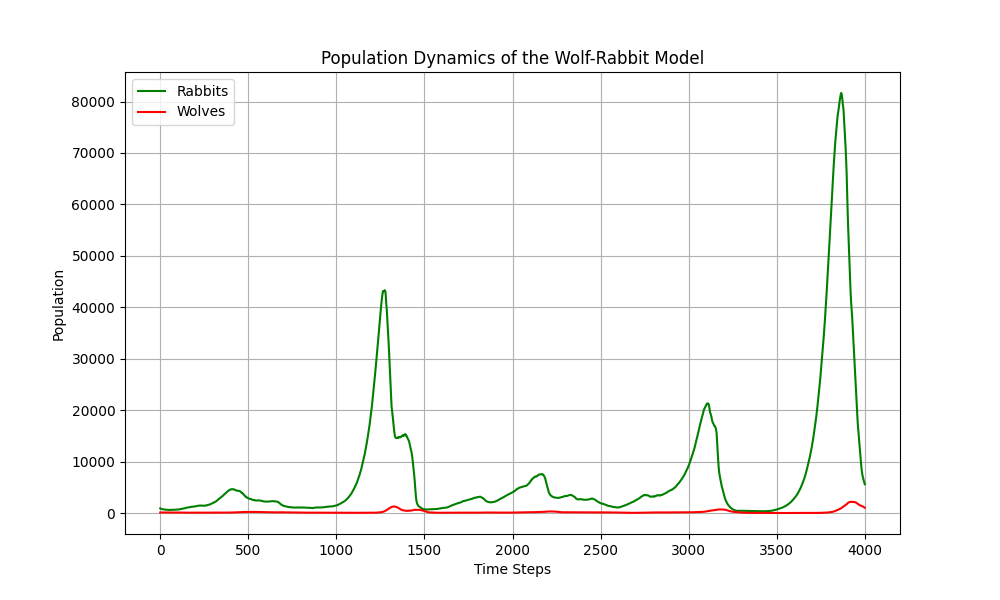
\includegraphics[width=\textwidth]{./media/population_dynamics_ex03.png}
	\caption{
		\textbf{Population Dynamics}
		$L = 8$, $\sigma = 0.05$
	}
	\label{fig:ex03}
\end{figure}

